\documentclass{article}

\usepackage{iclr2026_conference,times}
\input{math_commands.tex}

\usepackage{hyperref}
\usepackage{url}
\usepackage{booktabs}
\usepackage{graphicx}
\usepackage{amsmath}
\usepackage{amssymb}
\usepackage{microtype}
\graphicspath{{../figures/}}

\title{Cross-Embodiment Action Renormalization}

\author{Anonymous Authors}

\newcommand{\EJAR}{\mathrm{EJAR}}
\newcommand{\diag}{\mathrm{diag}}

\begin{document}

\maketitle

\begin{abstract}
Robot learning papers often report cross-embodiment transfer after normalizing each robot's action vector into a common numeric range. This quietly assumes that a normalized action coordinate has comparable physical meaning across bodies. We argue that this is the wrong invariant. Equal policy tokens should preserve local task effects, or at least preserve equal fractions of what each body can locally do. We propose Effect-Jacobian Action Renormalization (EJAR), a rule that encodes actions through the local action-to-task-effect map and decodes them through a target body's capability ellipsoid. EJAR is not a larger model, a new benchmark, or an uncertainty wrapper. It changes the central action variable: policy outputs become effect tokens with an explicit residual when a requested effect is infeasible. A 1000-paper automated landscape sweep and 100-paper hostile prior-work set locate the narrow novelty boundary: operational-space control already supplies much of the mathematics, but usually below the policy interface rather than as the shared cross-embodiment action representation. In planar-arm experiments with different link lengths, degrees of freedom, and actuator limits, raw normalized action copying has mean one-step relative effect error $1.25$, while EJAR absolute-effect decoding reduces it to $0.27$ and capability-token decoding to $0.016$. Transferred action-sequence success rises from $0.371$ to $0.792$. The evidence is deliberately small and mechanistic; the claim is that action normalization is a falsifiable physical assumption, not a harmless preprocessing step.
\end{abstract}

\section{Introduction}

Cross-embodiment robot learning is becoming a central bet in embodied intelligence. Robot foundation policies are trained on heterogeneous robot data \citep{openx2023,octo2024,kim2024openvla,brohan2023rt1,brohan2023rt2}, imitation systems represent long action chunks \citep{zhao2023act,chi2023diffusion}, and retargeting pipelines move demonstrations across hands, arms, tools, and mobile manipulators. These systems need a common action interface. A frequent engineering answer is to normalize each robot's commanded joint or end-effector coordinates to a shared range and let a policy, robot token, or controller absorb the remaining difference.

The hidden assumption is sharper than it looks: the number $0.4$ in an action coordinate is treated as if it has comparable task meaning on different bodies. For two arms at different configurations, the same normalized joint displacement can move the end effector in almost opposite directions. For a near-singular target, an apparently small source action may request a task effect the target cannot realize. Data scale can sometimes learn around this mismatch, but the action representation has already made the physical invariant ambiguous.

This paper asks a smaller question: what if the cross-embodiment action token were normalized by local task effect rather than by actuator coordinate? Let embodiment $e$ have configuration $q_e$, actuator step bounds $B_e$, task map $\phi_e(q_e)$, and local Jacobian $J_e(q_e)=\partial \phi_e/\partial q_e$. EJAR encodes a source action $a_e$ as the effect $d=J_e a_e$ or as a dimensionless capability token
\begin{equation}
z = \Sigma_e(q_e)^{-1/2}J_e(q_e)a_e,\quad
\Sigma_e(q_e)=J_e(q_e)B_e^2J_e(q_e)^\top.
\end{equation}
The target decodes either an absolute effect $d$ or a capability token $z$ by a damped minimum-energy pullback through its own local Jacobian and limits. The residual after clipping is part of the output, not an afterthought.

Our contributions are:
\begin{itemize}
\item A hostile literature boundary for cross-embodiment action transfer, produced from a 1000-paper sweep, a 300-paper serious skim, a 240-paper deep-read subset, and a 100-paper hostile prior set.
\item EJAR, a mechanism that renormalizes cross-body actions by local task effects and local capability ellipsoids.
\item A first-order preservation proposition that states exactly when the rule works and where clipping, singularities, and task-map mismatch break it.
\item Runnable synthetic evidence showing that raw action normalization fails even in planar arms, while EJAR substantially reduces one-step effect error and trajectory-tracking error.
\end{itemize}

The paper is intentionally honest about scope. EJAR does not solve perception, correspondence, contact-mode selection, or real hardware calibration. It is a mechanism and diagnostic for the action variable used by cross-embodiment policies.

\section{Related Work and Novelty Boundary}

\paragraph{Robot foundation policies.}
Large robot policies such as RT-1, RT-2, Open X-Embodiment/RT-X, Octo, RoboCat, and OpenVLA scale behavior cloning or sequence modeling across many tasks and robots \citep{brohan2023rt1,brohan2023rt2,openx2023,octo2024,li2023robocat,kim2024openvla}. These works make cross-robot data useful, but their action interfaces still need a decoding convention. EJAR is complementary: it can be used as an action layer before training or as a diagnostic for whether a shared model output has comparable physical meaning.

\paragraph{Action sequence policies and imitation.}
Diffusion Policy, ACT, PerAct, Transporter Networks, and offline imitation systems improve how policies represent temporally extended actions \citep{chi2023diffusion,zhao2023act,shridhar2023peract,florence2020transporter,mandlekar2021robomimic}. These papers usually study policy architecture, visual representation, or demonstration learning, not whether a normalized action token preserves the same differential task effect when decoded by another body.

\paragraph{Control and kinematics.}
Resolved-rate control and operational-space control already map desired task motion through robot Jacobians \citep{whitney1969resolved,khatib1987operational}. This is the closest hostile prior work. We do not claim that the weighted pseudoinverse is new as a controller. The novelty boundary is the use of the local effect map to define the shared cross-embodiment \emph{policy action variable} and to expose an infeasibility residual at the data/model interface.

\paragraph{Benchmarks and datasets.}
RLBench, Meta-World, RoboNet, BridgeData V2, and related datasets support robot manipulation evaluation at scale \citep{james2020rlbench,yu2020meta,dasari2019robonet,walke2023bridgedata}. EJAR is not a benchmark. Its role is to test and repair a hidden assumption that can appear inside such benchmarks when demonstrations or policy outputs are mapped across robots.

\paragraph{Automated hostile sweep.}
We queried OpenAlex for cross-embodiment learning, robot action representations, retargeting, morphology transfer, task-space control, robot foundation policies, manipulation, sim-to-real, and related embodied-intelligence terms. We ranked 1000 entries by relevance and citations, annotated every row with claimed problem, mechanism, hidden assumptions, fixed variables, ignored failure modes, novelty impact, and open questions, then used the top 100 as hostile priors. The sweep is abstract-level and therefore imperfect. Its purpose is adversarial coverage, not final citation scholarship. The generated artifacts are in \texttt{docs/related\_work\_matrix.csv}, \texttt{docs/literature\_map.md}, and \texttt{docs/hostile\_prior\_work.md}.

\section{Effect-Jacobian Action Renormalization}

Let $q_e\in\R^{n_e}$ be the configuration of embodiment $e$, and let $a_e\in\R^{n_e}$ be a small low-level action such as a joint-position or joint-velocity increment over one control period. Let $\phi_e(q_e)\in\R^m$ be the task variable to preserve, for example end-effector displacement or an object-centric local coordinate. Its local action-to-effect map is
\begin{equation}
d_e = \phi_e(q_e+a_e)-\phi_e(q_e)\approx J_e(q_e)a_e.
\end{equation}
Let $B_e=\diag(b_e)$ contain per-coordinate action limits for one step. The local effect-capability ellipsoid is
\begin{equation}
\Sigma_e(q_e)=J_e(q_e)B_e^2J_e(q_e)^\top.
\end{equation}
This matrix says which task-space directions the body can affect strongly at $q_e$. It changes with configuration, not just with morphology.

\paragraph{Absolute-effect decoding.}
If a source demonstration supplies a desired local effect $d$, the target action is
\begin{equation}
\EJAR_e(d;q_e)=B_e^2J_e(q_e)^\top\left(J_e(q_e)B_e^2J_e(q_e)^\top+\lambda I\right)^{-1}d,
\end{equation}
followed by proportional clipping to respect $B_e$. The target also reports the residual
\begin{equation}
r_e=\left\|J_e(q_e)\EJAR_e(d;q_e)-d\right\|_2.
\end{equation}
A large residual is not a failure of bookkeeping; it is evidence that the requested transfer is not locally feasible.

\paragraph{Capability-token decoding.}
For a policy that should output a dimensionless cross-body token, EJAR uses
\begin{equation}
z_e(a_e;q_e)=\left(\Sigma_e(q_e)+\epsilon I\right)^{-1/2}J_e(q_e)a_e.
\end{equation}
Decoding $z$ on target $t$ requests the locally normalized effect
\begin{equation}
d_t=\left(\Sigma_t(q_t)+\epsilon I\right)^{1/2}z,
\end{equation}
then applies absolute-effect decoding. Equal tokens mean equal fractions of each robot's local effect capability, not necessarily equal metric displacements. This distinction matters: absolute-effect transfer is appropriate when the target must reproduce a source task displacement; capability-token transfer is appropriate when the policy should command comparable local authority across bodies.

\paragraph{Proposition.}
Assume first-order dynamics, no clipping, $\lambda=0$, and $J_eB_e$ has full row rank. Then for every desired effect $d\in\R^m$,
\begin{equation}
J_e(q_e)\EJAR_e(d;q_e)=d.
\end{equation}
For capability tokens, the decoded action satisfies
\begin{equation}
J_e(q_e)\EJAR_e\left(\Sigma_e(q_e)^{1/2}z;q_e\right)=\Sigma_e(q_e)^{1/2}z.
\end{equation}
\emph{Proof.} Substitute the definition. Since $\Sigma_e=J_eB_e^2J_e^\top$ is invertible under full row rank,
\begin{equation}
J_eB_e^2J_e^\top\left(J_eB_e^2J_e^\top\right)^{-1}d=d.
\end{equation}
The token claim follows by setting $d=\Sigma_e^{1/2}z$. \hfill $\square$

The proposition is intentionally local. Damping introduces a residual, clipping breaks exact preservation, and a wrong task map invalidates the premise.

\section{Synthetic Evidence}

\paragraph{Setup.}
We use a planar 2-link teacher arm and three target arms: a shorter 2-link arm, a longer 2-link arm with smaller joint limits, and an asymmetric 3-link arm. For each randomized source configuration and source action, we compute the source first-order end-effector effect. Targets receive either (i) raw normalized joint action copying, padding or truncating dimensions as needed; (ii) EJAR absolute-effect decoding; or (iii) EJAR capability-token decoding. We also run short transferred action sequences, where the target tries to follow the cumulative source effect trajectory. Every thirteenth one-step trial and every seventeenth trajectory episode uses a near-singular target configuration to stress the residual boundary.

\begin{table}[t]
\centering
\caption{One-step cross-body effect transfer over 9600 method trials. Lower relative error is better; higher cosine is better.}
\label{tab:onestep}
\begin{tabular}{lccc}
\toprule
Method & Mean rel. error & Median rel. error & Mean cosine \\
\midrule
Raw normalized copy & 1.252 & 1.212 & 0.038 \\
EJAR absolute effect & 0.265 & 0.087 & 0.973 \\
EJAR capability token & 0.016 & 0.005 & 0.998 \\
\bottomrule
\end{tabular}
\end{table}

\begin{figure}[t]
\centering
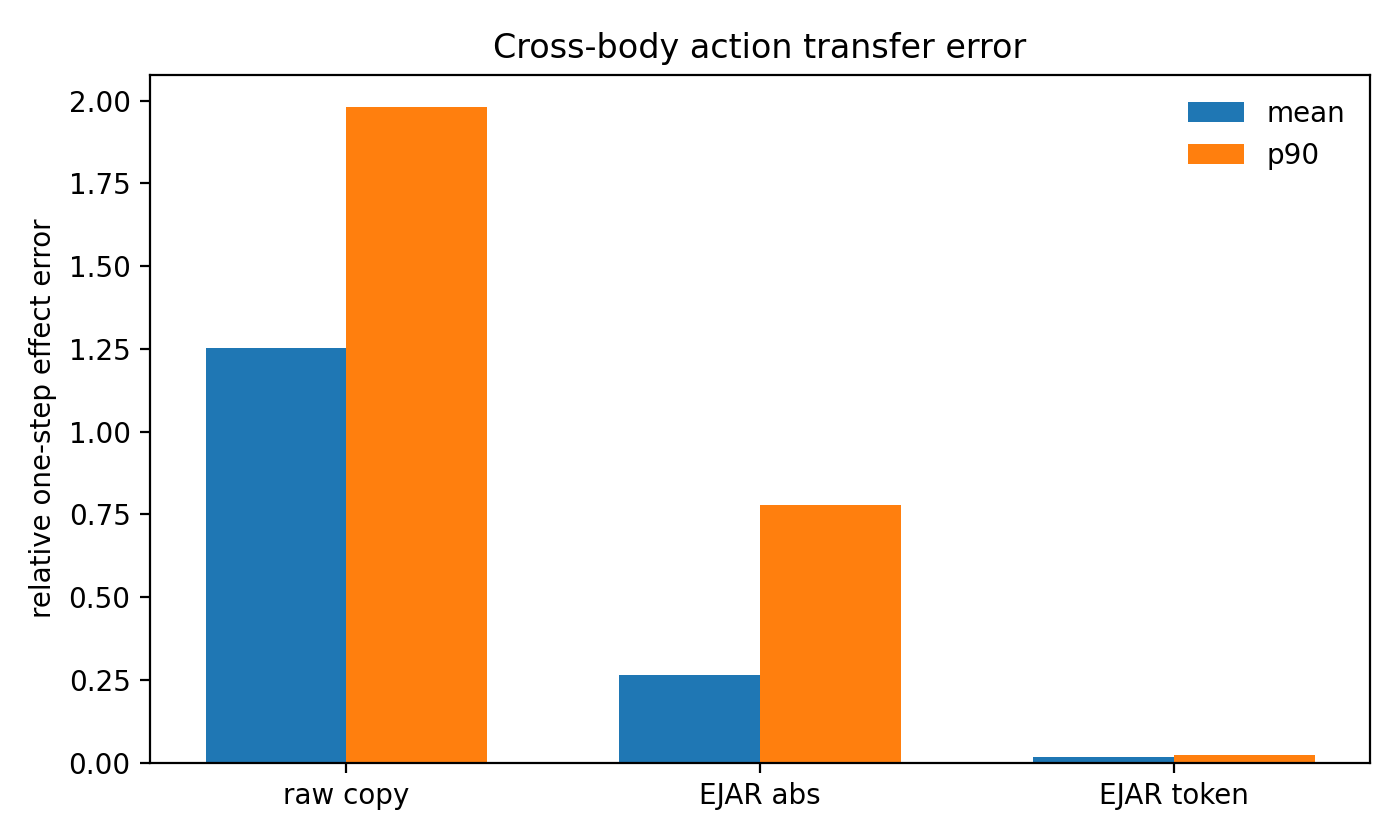
\includegraphics[width=0.68\linewidth]{one_step_effect_error.png}
\caption{Raw componentwise action copying does not preserve local task effects across bodies. EJAR reduces one-step effect error, and the token mode preserves normalized local capability most tightly.}
\label{fig:onestep}
\end{figure}

\begin{table}[t]
\centering
\caption{Transferred source action sequences over 480 method episodes. Success means final tracking error below 0.10 workspace units.}
\label{tab:trajectory}
\begin{tabular}{lccc}
\toprule
Method & Mean final error & Median final error & Success \\
\midrule
Raw normalized copy & 0.181 & 0.137 & 0.371 \\
EJAR absolute effect & 0.065 & 0.043 & 0.792 \\
\bottomrule
\end{tabular}
\end{table}

\begin{figure}[t]
\centering
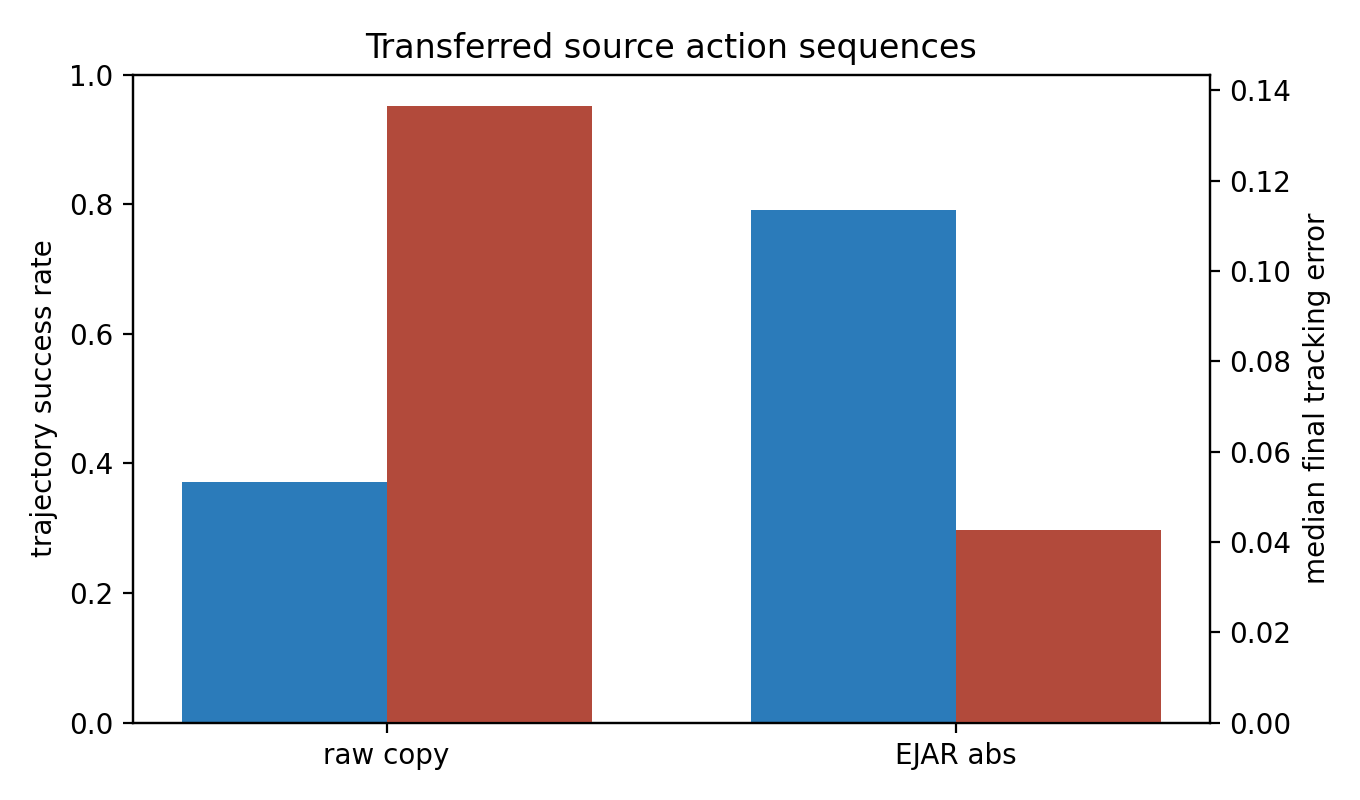
\includegraphics[width=0.65\linewidth]{trajectory_transfer.png}
\caption{On short action sequences, EJAR substantially improves target tracking of the source's cumulative task effects.}
\label{fig:trajectory}
\end{figure}

\paragraph{Readout.}
The experiment supports the narrow claim. Raw normalized joint copying is not a cross-body effect invariant. EJAR absolute decoding substantially improves effect preservation, but its mean error remains nonzero because some source effects are infeasible for a target at its configuration or under its limits. Capability-token decoding has very low normalized token error because it asks each target to realize the same fraction of its own local capability ellipsoid. These are different promises, and the paper separates them.

\section{Limitations}

EJAR assumes a chosen task map $\phi$, a local Jacobian, actuator-step limits, and a regime where first-order effects are meaningful. Those assumptions can fail in contact-rich manipulation, under latency, with unmodeled compliance, or when the source and target do not share a valid task correspondence. The method does not estimate Jacobians, learn visual policies, choose contact modes, or solve nullspace objectives. The literature sweep is automated and should be treated as a hostile map, not as a substitute for manual reading. The evidence is synthetic. A submit-ready full paper would need real multi-robot demonstrations or logged heterogeneous robot datasets.

\section{Conclusion}

Cross-embodiment learning should not treat action normalization as an implementation detail. A shared action token is a physical claim about what should be preserved across bodies. EJAR makes that claim explicit: preserve local task effects when feasible, or preserve equal fractions of local capability when a dimensionless token is required, and report the residual when the request is impossible. The result is modest but useful: a central mechanism, a formal local boundary, and runnable evidence that the common componentwise normalization assumption can be false.

\bibliography{references}
\bibliographystyle{iclr2026_conference}

\appendix

\section{Reproducibility}

The repository contains the literature generator, synthetic experiment, generated CSVs, figures, and this paper source. The main experiment command is:
\begin{verbatim}
python experiments/run_ejar_synthetic.py
\end{verbatim}
The literature command is:
\begin{verbatim}
python scripts/generate_literature.py
\end{verbatim}
The final paper build uses direct pdfLaTeX/BibTeX passes from the \texttt{paper/} directory.

\section{Assumptions Broken During Direction Selection}

The novelty decision considered more than twenty assumptions, including: normalized joint deltas are comparable across link lengths; end-effector displacement is equally feasible across configurations; action frequency is irrelevant; robot identity tokens can absorb local action-map mismatch; retargeting poses is equivalent to retargeting effects; workspace overlap is enough; nullspace motion is harmless; simulation randomization covers action-effect anisotropy; and closed-loop correction makes one-step mismatch unimportant. The full list is in \texttt{docs/novelty\_boundary\_map.md}.

\section{Reviewer-Facing Weaknesses}

The strongest attack is that EJAR reuses operational-space mathematics. We agree and state the boundary narrowly: the controller primitive is old, while the proposed contribution is to use the local effect map as the cross-embodiment policy/data action representation and infeasibility diagnostic. The second strongest attack is weak evidence. We also agree: this is a mechanism paper with synthetic evidence and should be revised with real robot logs before a full conference submission.

\end{document}
